%=======================02-713 LaTeX template, following the 15-210 template==================
%
% You don't need to use LaTeX or this template, but you must turn your homework in as
% a typeset PDF somehow.
%
% How to use:
%    1. Update your information in section "A" below
%    2. Write your answers in section "B" below. Precede answers for all 
%       parts of a question with the command "\question{n}{desc}" where n is
%       the question number and "desc" is a short, one-line description of 
%       the problem. There is no need to restate the problem.
%    3. If a question has multiple parts, precede the answer to part x with the
%       command "\part{x}".
%    4. If a problem asks you to design an algorithm, use the commands
%       \algorithm, \correctness, \runtime to precede your discussion of the 
%       description of the algorithm, its correctness, and its running time, respectively.
%    5. You can include graphics by using the command \includegraphics{FILENAME}
%
\documentclass[11pt]{article}

\usepackage{amsmath,amssymb,amsthm}
\usepackage{graphicx}
\usepackage[margin=1in]{geometry}
\usepackage{fancyhdr}
\usepackage{comment}
\usepackage{tikz}
\usetikzlibrary{arrows}
\usepackage{caption}
\usepackage{subcaption}


\setlength{\parindent}{0pt}
\setlength{\parskip}{5pt plus 1pt}
\setlength{\headheight}{13.6pt}
\newcommand\question[2]{\vspace{.25in}\hrule\textbf{#1: #2}\vspace{.5em}\hrule\vspace{.10in}}
\renewcommand\part[1]{\vspace{.10in}\textbf{(#1)}}
\newcommand\algorithm{\vspace{.10in}\textbf{Algorithm: }}
\newcommand\correctness{\vspace{.10in}\textbf{Correctness: }}
\newcommand\runtime{\vspace{.10in}\textbf{Running time: }}
\pagestyle{fancyplain}
\lhead{\textbf{\NAME\ \ANDREWID}}
\chead{\textbf{Assignment\HWNUM}}
\rhead{CS 440, Winter 2018}
\begin{document}\raggedright
%Section A==============Change the values below to match your information==================
\newcommand\NAME{Thomas Noelcke}  % your name
\newcommand\ANDREWID{noelcket}     % your andrew id
\newcommand\HWNUM{2}              % the homework number
%Section B==============Put your answers to the questions below here=======================

% no need to restate the problem --- the graders know which problem is which,
% but replacing "The First Problem" with a short phrase will help you remember
% which problem this is when you read over your homeworks to study.

The assignment is to be turned in before Midnight (by 11:59pm) on January 25th, 2018. 
You should turn in the solutions to this assignment as a pdf file through the TEACH website.
The solutions should be produced using editing software programs, such as LaTeX or Word, otherwise they will not be graded.
Trees can be drawn on paper and scanned.


\question{1}{File Structures (1 point)}
\begin{enumerate}
\item Consider a file with a large number of \textit{Customer(id, name, birth-date)} records. Assume that users frequently search this file based on a the field \textit{id} to find the values of \textit{name} or \textit{birth-date} for customers whose information is stored in the file. Moreover, assume that users rarely update current records or insert new records to the file. Which file structure, heap versus sorted, provides the fastest total running time for users' queries over this file? Explain your answer (0.5 point).\\

For this example the best file structure would be a sorted file structure sorted based on the ID of the Customer record. I would choose this file structure because a sorted file structure offers better run time efficiency for search type operations. This file structure does have some disadvantages when it comes to writing to the file structure however as indicated in the question we don't expect this operation to happen often.\\

\item Consider a file with a large number of \textit{Transaction(id, customerID, productID, amount)} records, which keeps track of the purchases made by a customer on various products. Assume that users frequently insert new records into this file. Users also query this file to compute the total amount of money each customer has spent on her purchases, similar to a SQL query with {\it Group By customerID}. Which file structure, heap versus sorted, provides the fastest total running time for users' queries over this file?  Explain your answer (0.5 point).

In this instance I would probably use a heap type files structure. As indicated by the question there will be a large number of records added to this file. A heap type file structure will offer the best performance when it comes to writing to the file. However, this file structure will be slower at querying using a group by statement as mentioned in the question prompt. However, if you are using a group by statement you are probably reading a decent amount of the records in the file any ways and likely wont suffer enough to justify giving up the write performance of a heap file structure.\\

\end{enumerate}

\question{2}{B+ Tree Indexing (2 points)}
Consider the B+ tree index shown in Figure~\ref{figure:q2}. 
Each intermediate node can hold up to five pointers and four key values. Each leaf can hold up to four pointers to data, and leaf nodes are doubly linked as usual, although these links are not shown in the figure.
Answer the following questions.\\


\begin{comment}
{"keys": [25,55,75],
 "children": [{"keys": [5,10,15,20]}, {"keys": [25,28,30,50]}, {"keys": [55,60,65,70]}, {"keys": [75,80,85,90]}]
}
\end{comment}

\begin{enumerate}
	\item Show the B+ tree that would result from inserting a record with search key 95 into the tree.
	\paragraph{solution:} \hfill \break
	See the graphic below for the solution to this problem.\\
	
	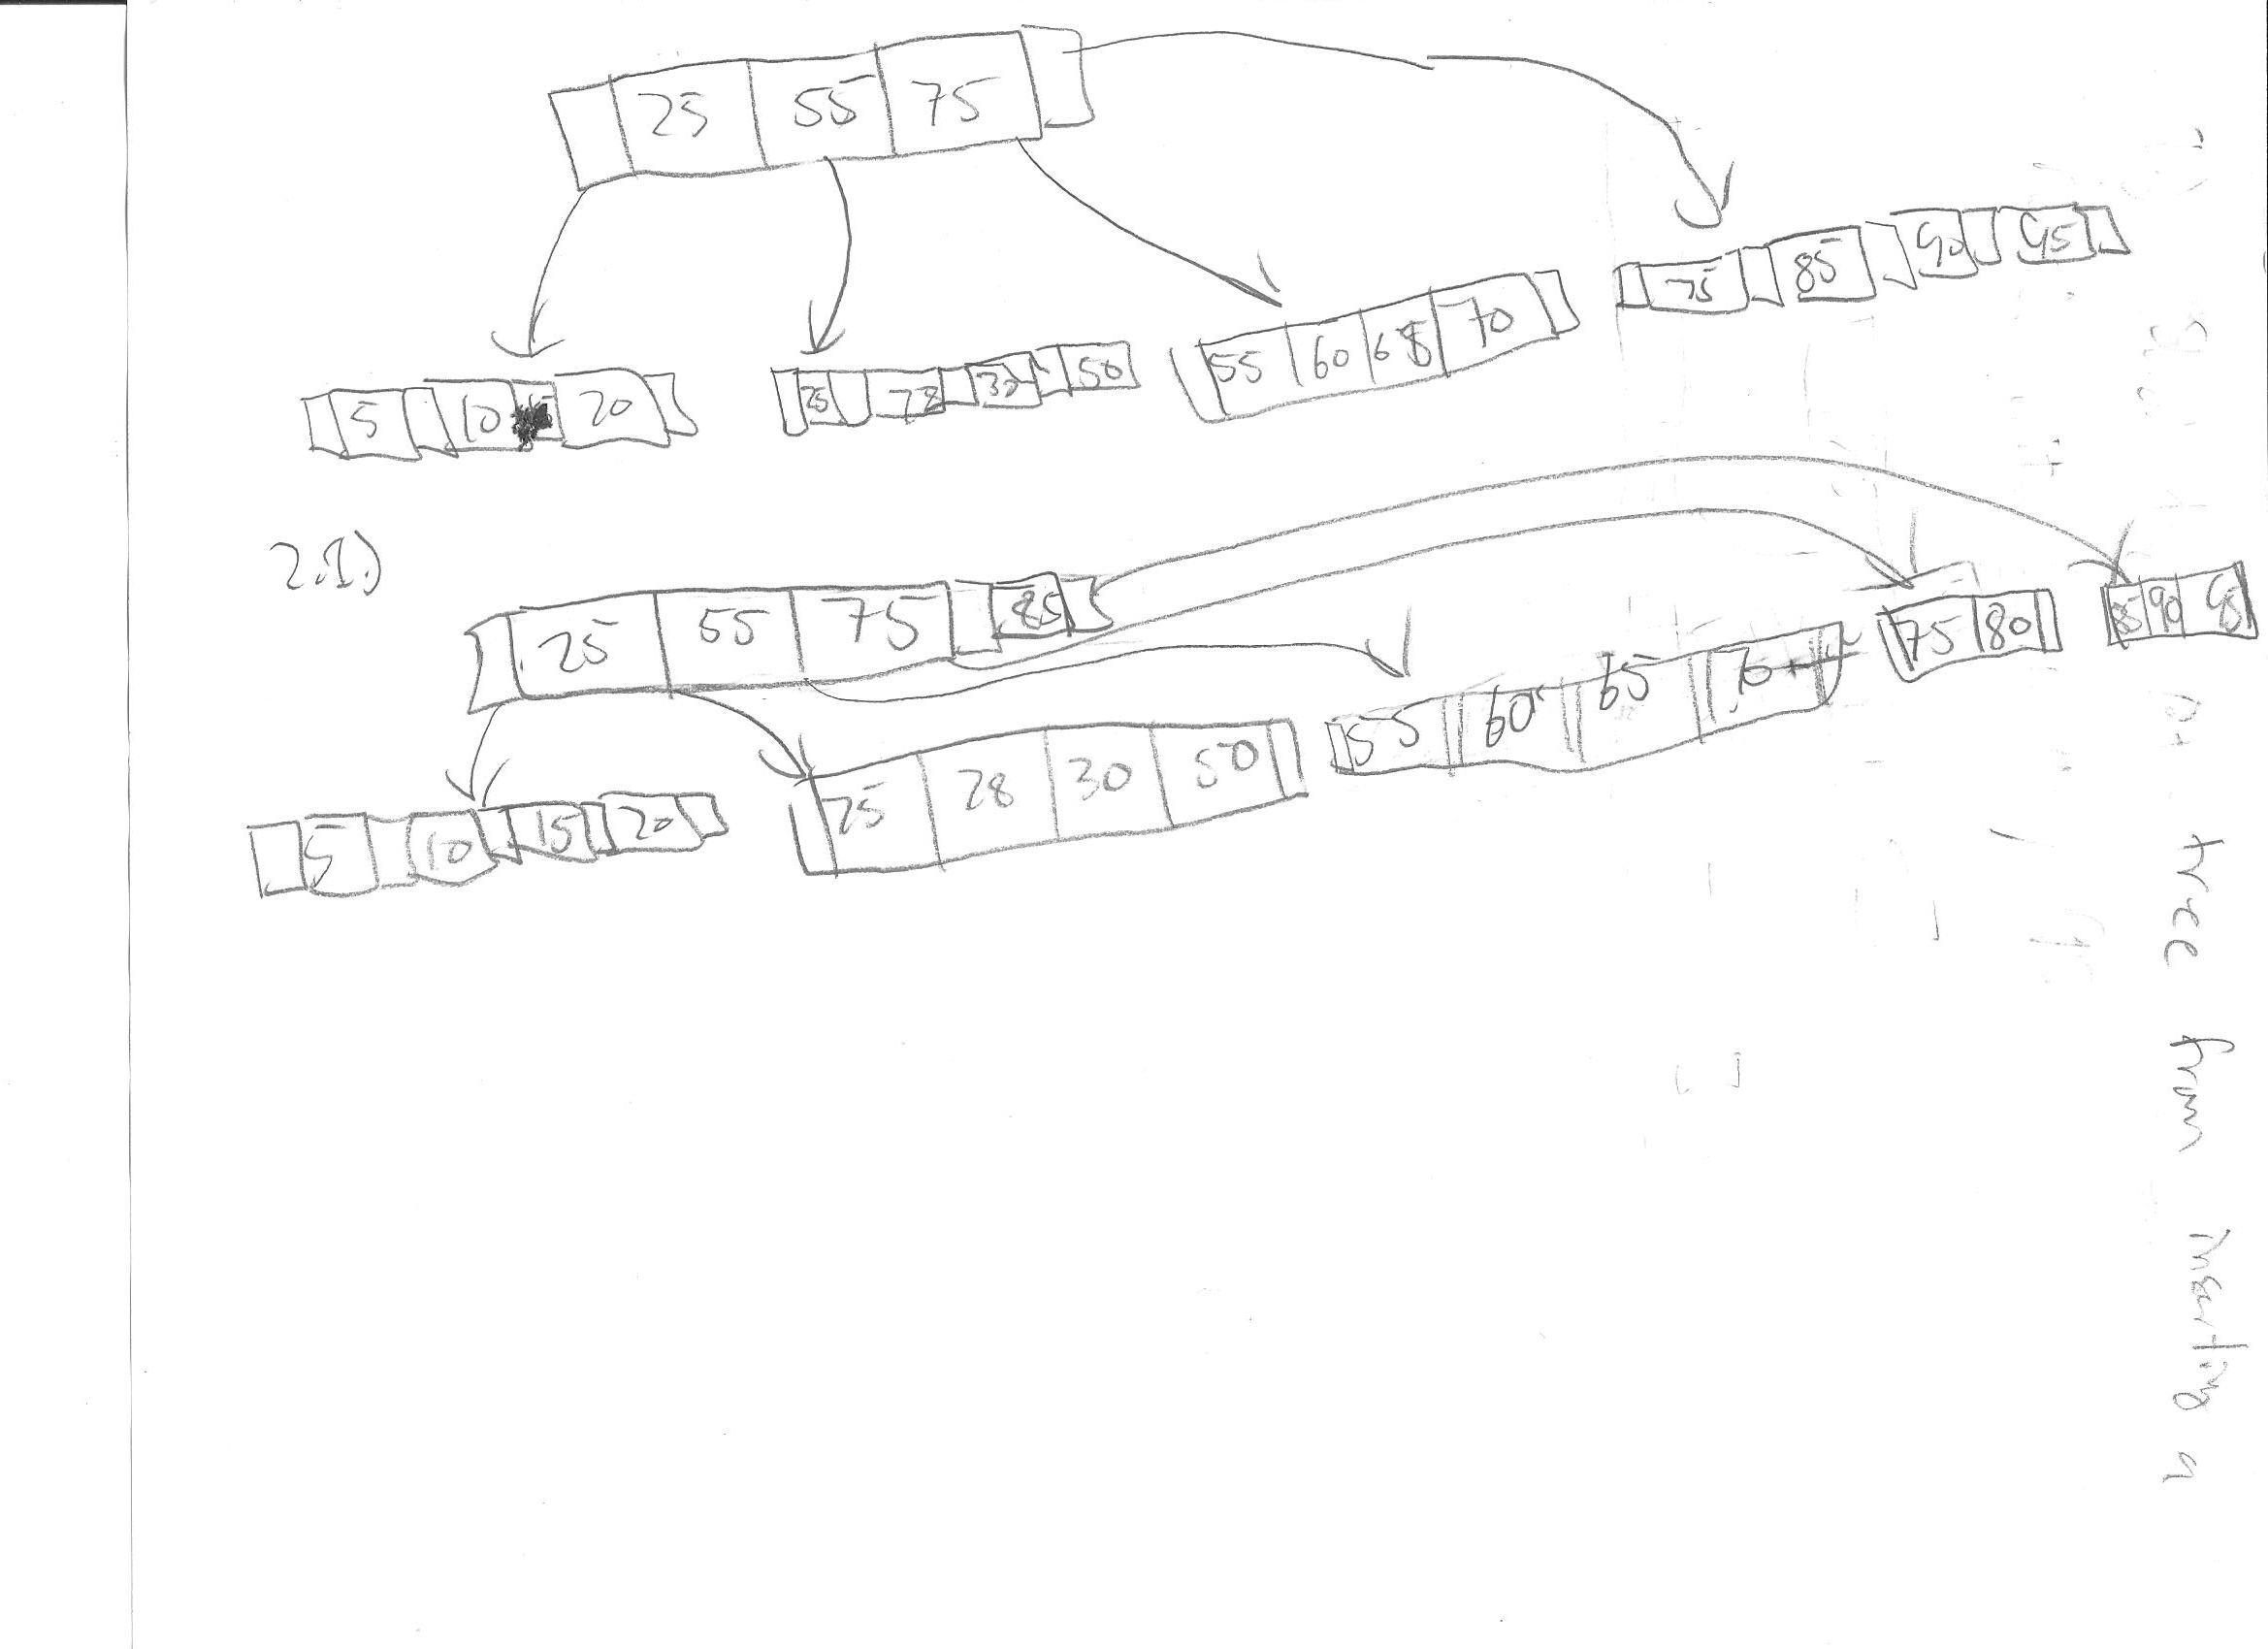
\includegraphics{twoPointOne.png}

	\item Use the result/solution tree from (1) and Show the B+ tree that would result from deleting the record with search key 60.
		\paragraph{solution:} \hfill \break
		See graphic below for solution.\\
		
		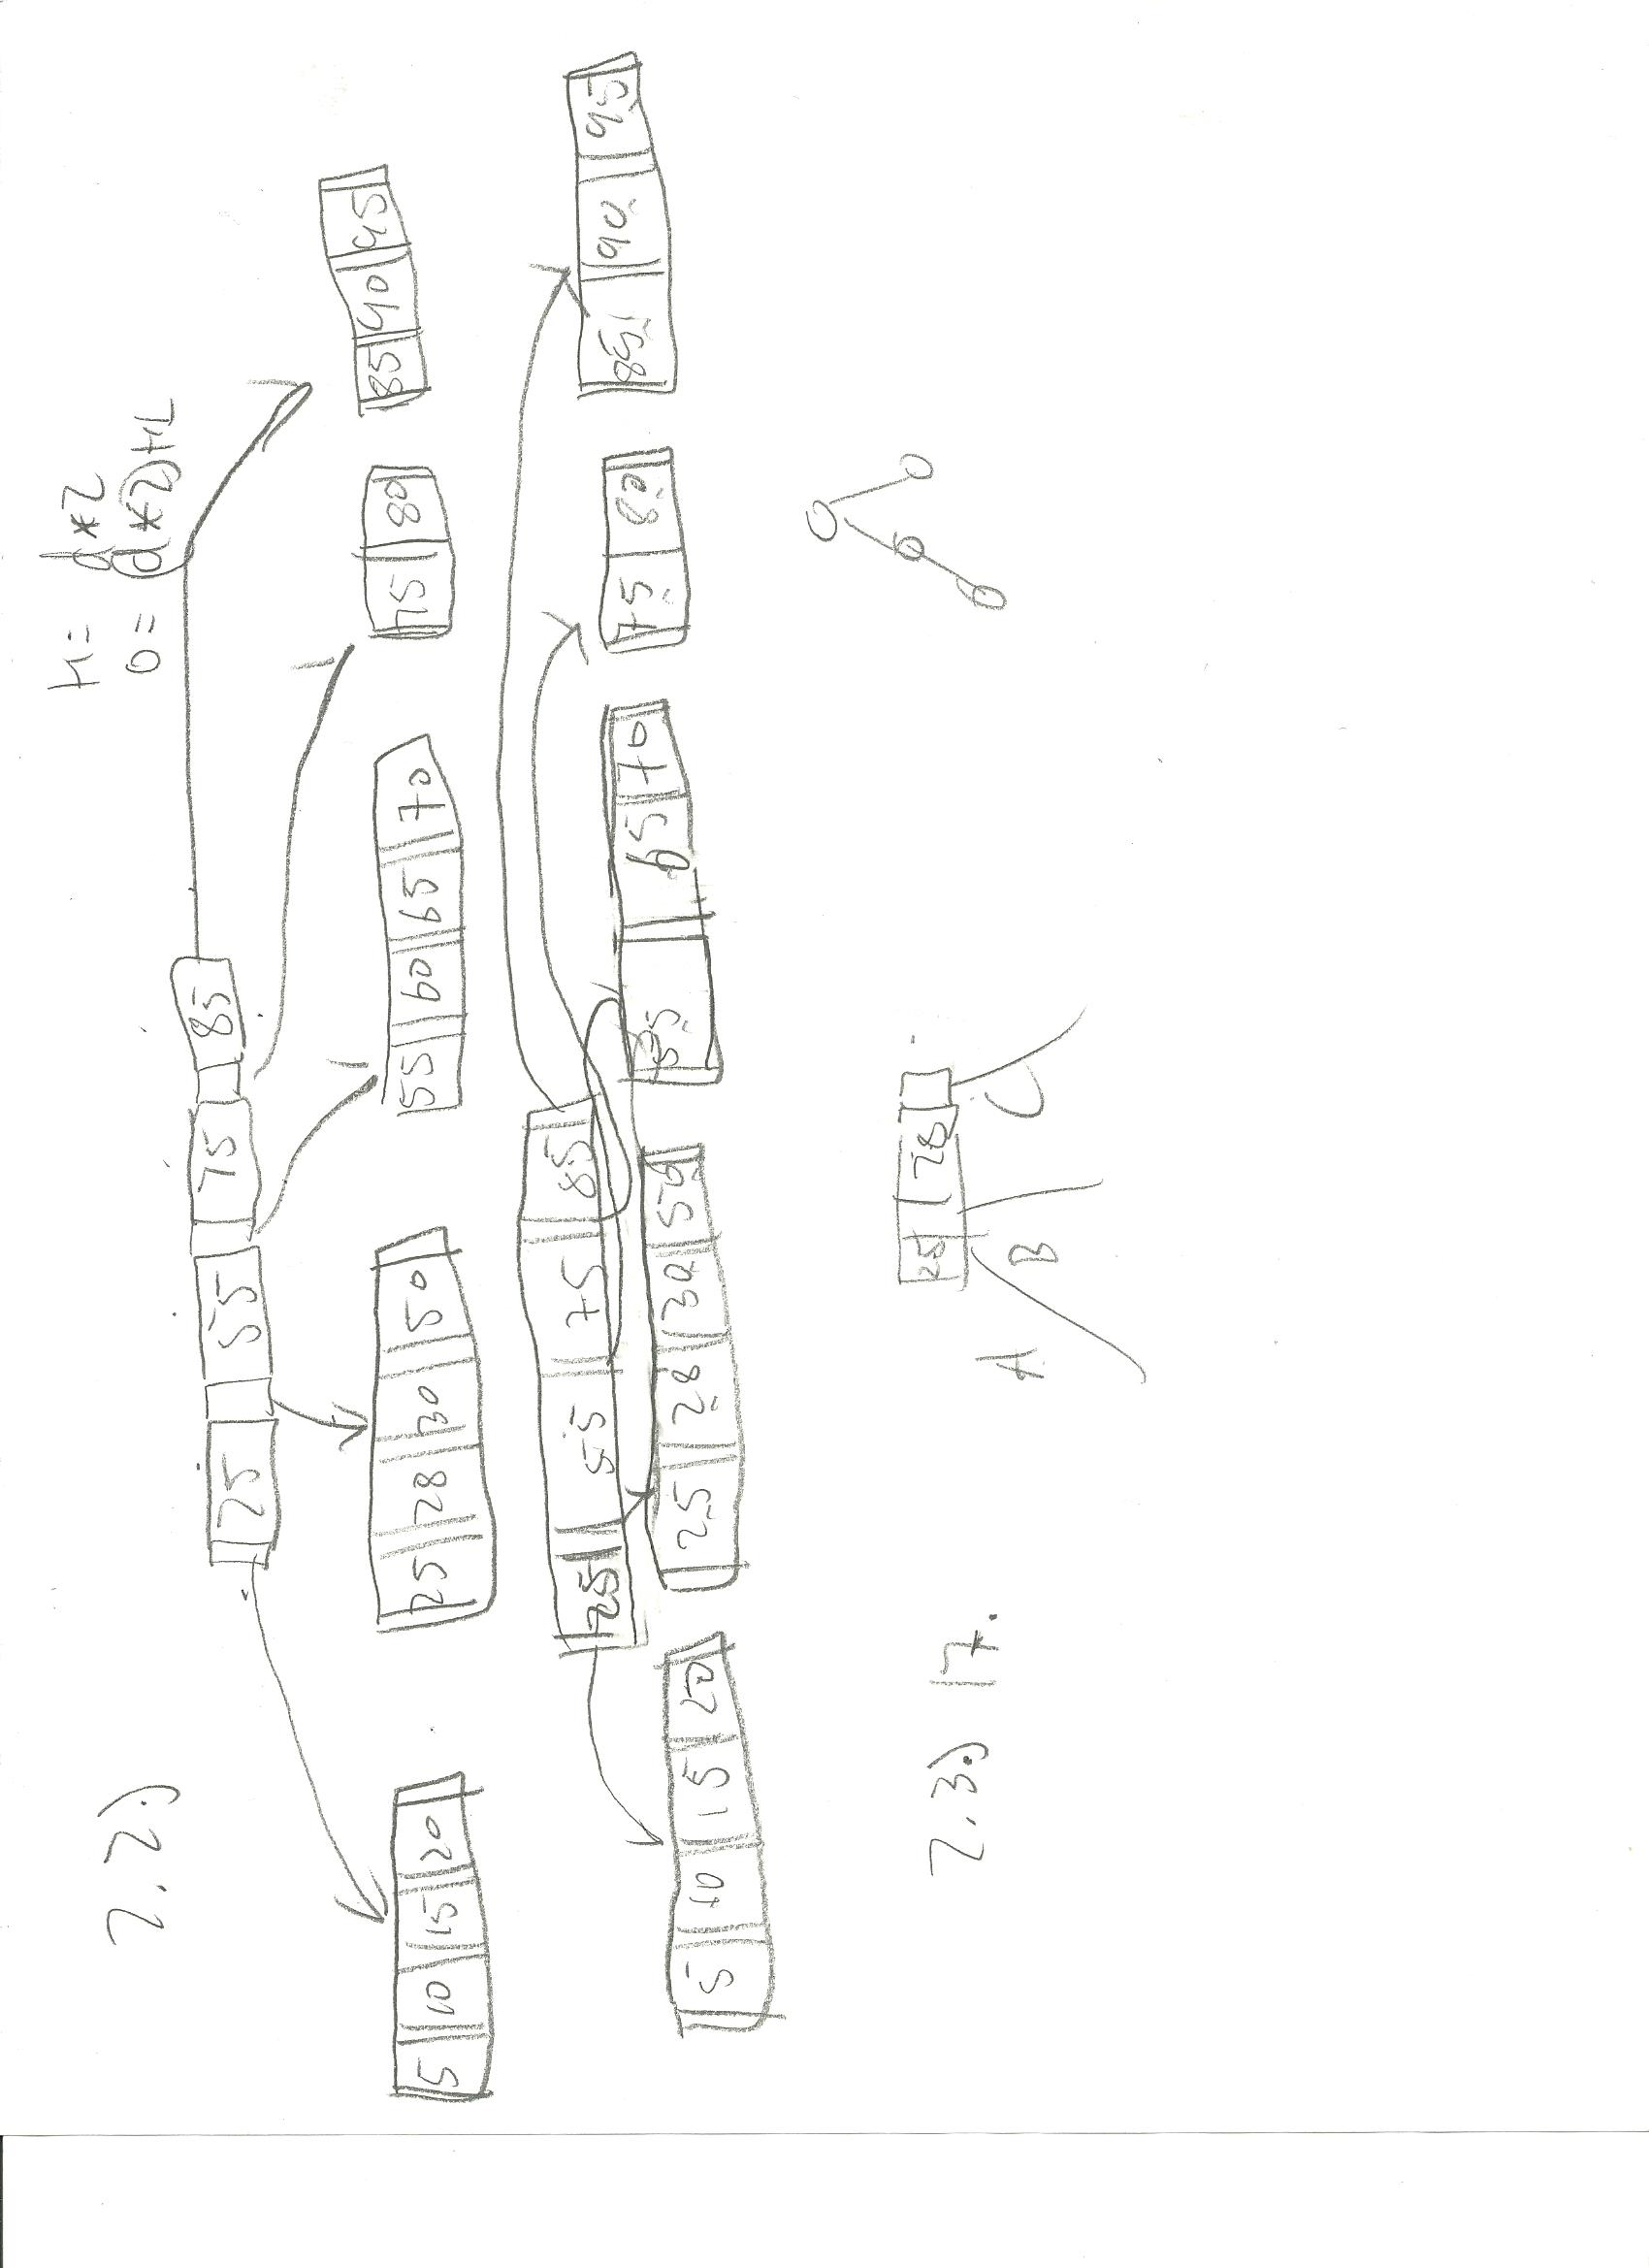
\includegraphics{twoPointTwo.jpeg}

	\item Name a search key value such that inserting it into the result/solution tree from (1) would cause an increase in the height of the tree.
	\paragraph{solution:} \hfill \break
	If you insert a value into either the left most or second to left most node (Between 5 and 30) would cuase hight to be added to the tree.\\

	\item What can you infer about the contents and the shape of A, B and C subtrees?
	\paragraph{solution}: \hfill \break
	We know that the A will contain values less than 10. We also know that b will contain key values between 10 and 19 and C will contain values between 20 and 29. We can also say that A, B and C must be leaf's because the tree must be balanced. Finally, we can say that each node must have between 2 and 4 keys and can at most have 5 pointers.\\
	
\end{enumerate}




\question{3}{B+ Tree Indexing (1 point)}
Suppose that a block can contain at most four data values and that all data values are integers. Using only B+ trees of degree 2, give examples of each of the following:
\begin{enumerate}
	\item A B+ tree whose height changes from 2 to 3 when the value 60 is inserted. Show your structure before and after the insertion.
	
	solution is shown below in graphic.\\
	
	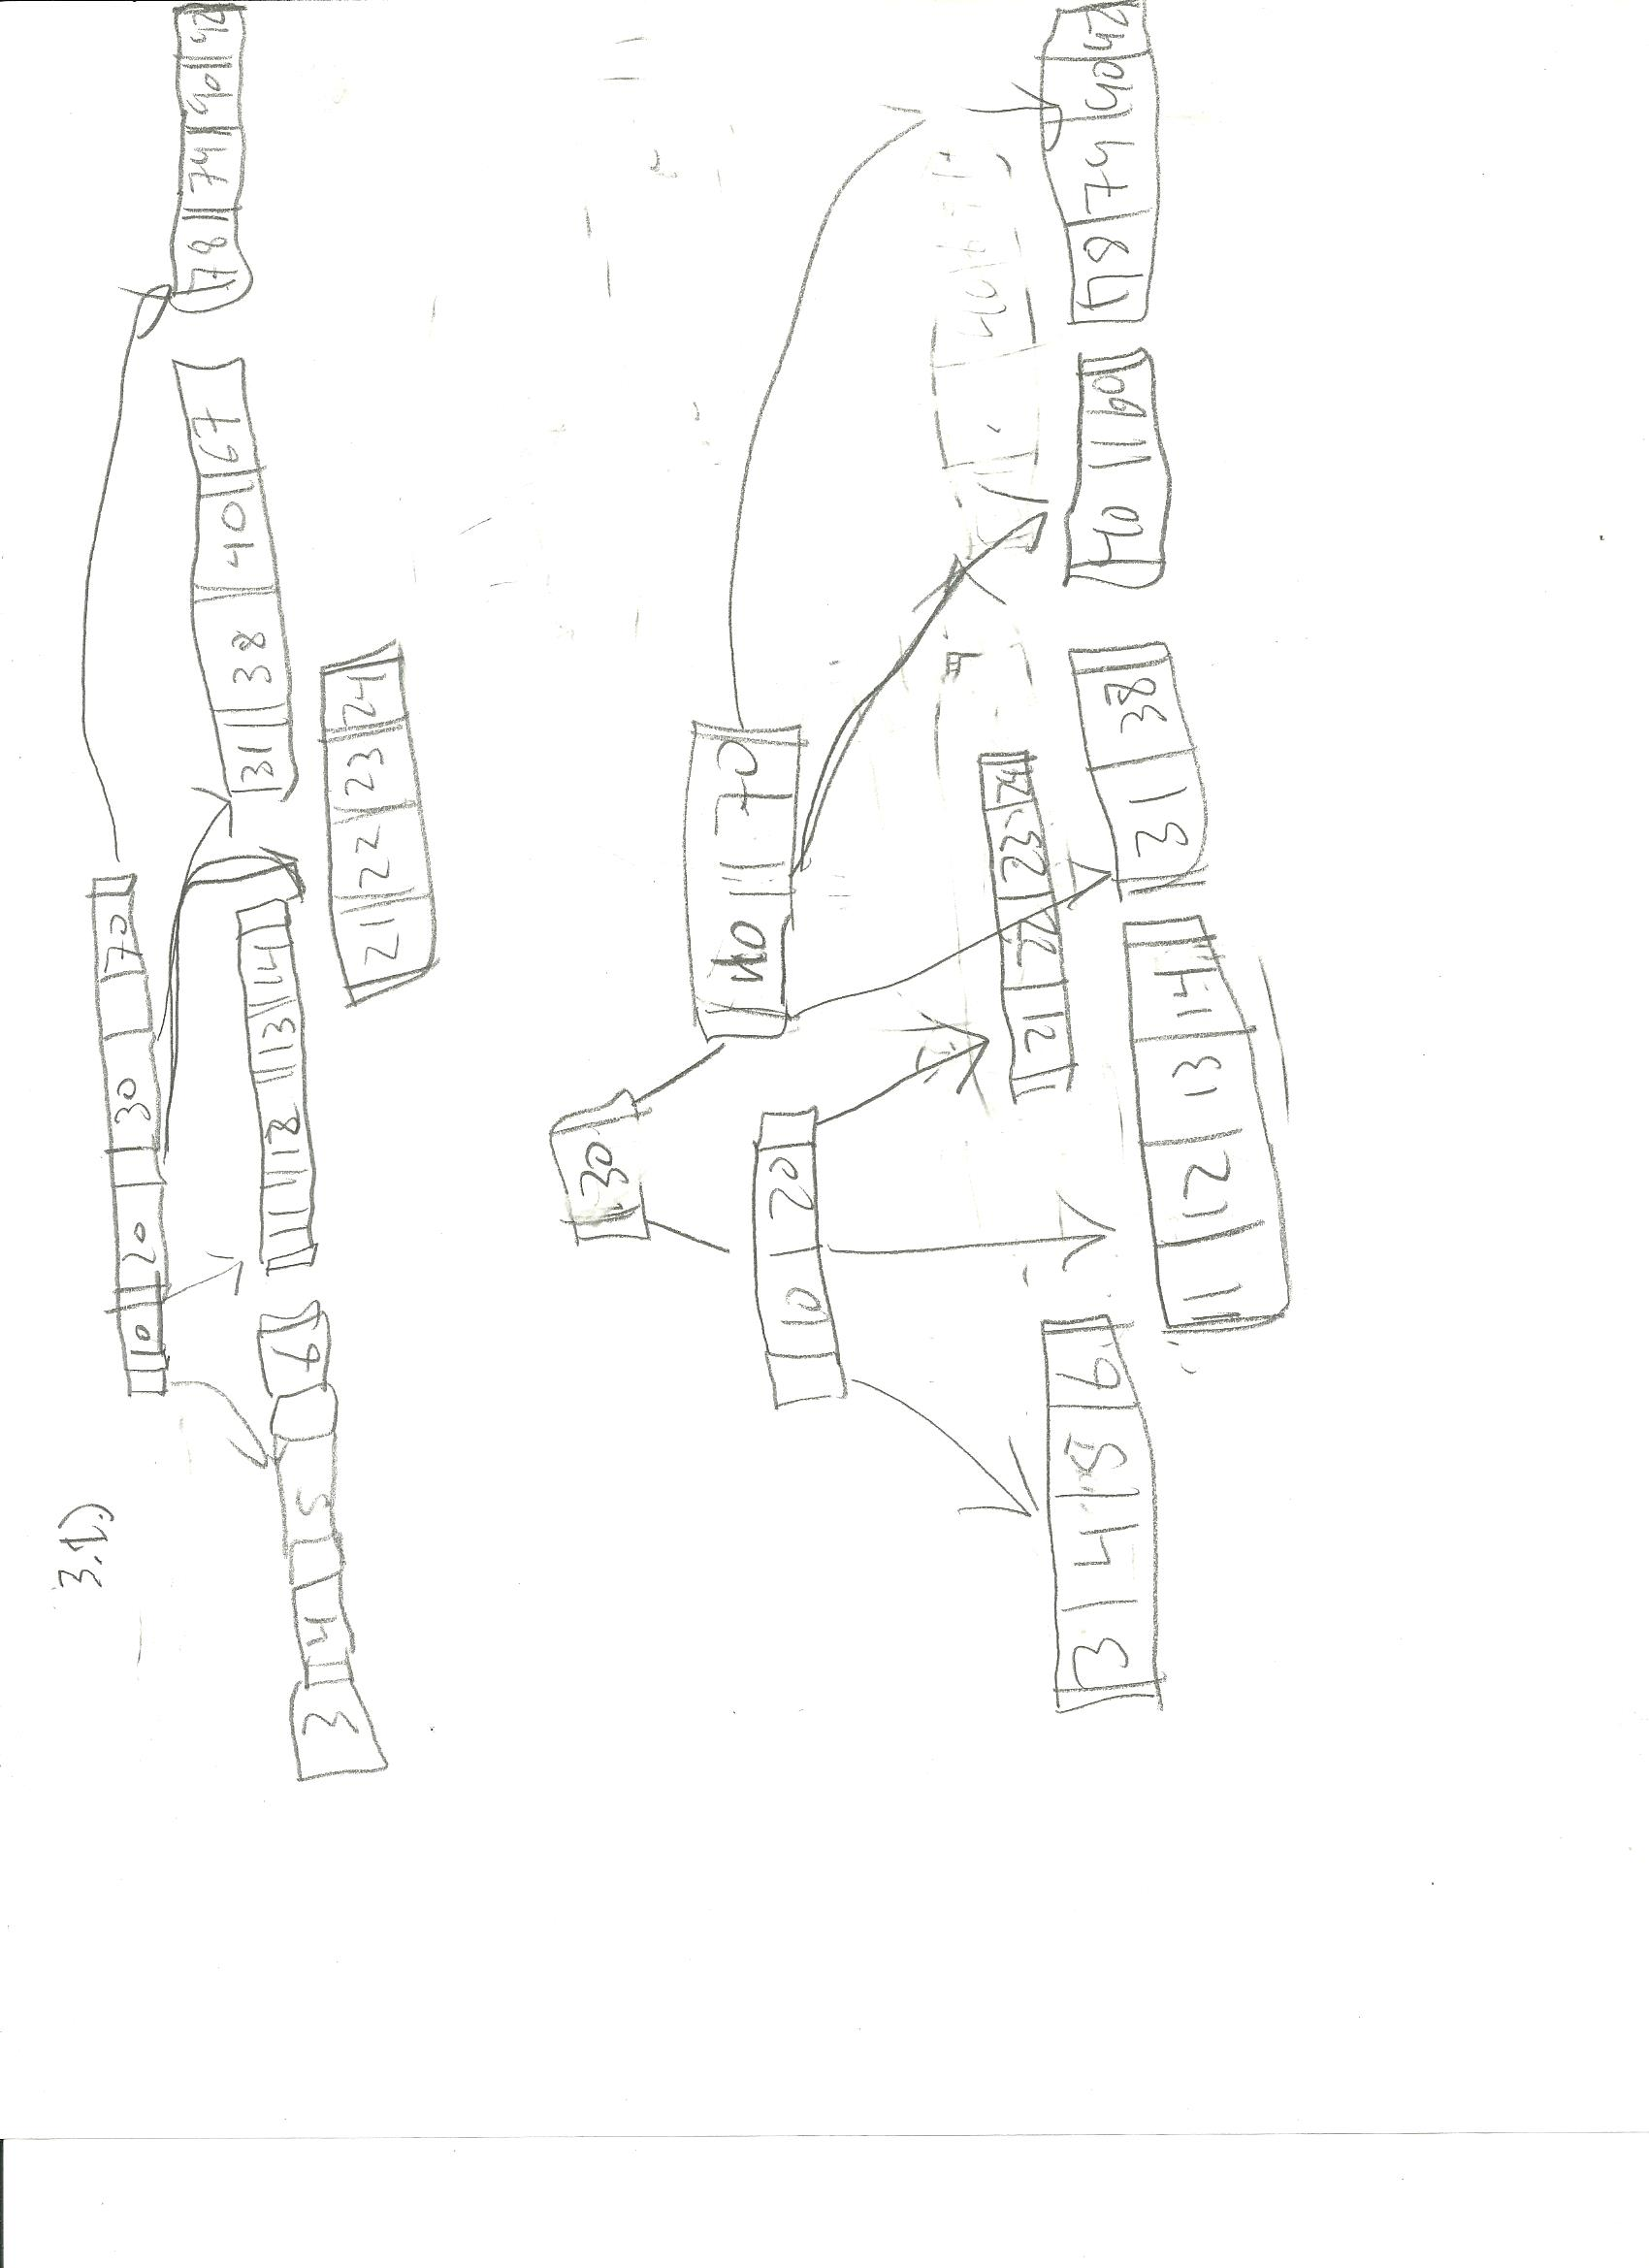
\includegraphics{threePointOne.jpeg}
	
	\item A B+ tree in which the deletion of the value 60 leads to a redistribution. Show your structure before and after the deletion.
	
	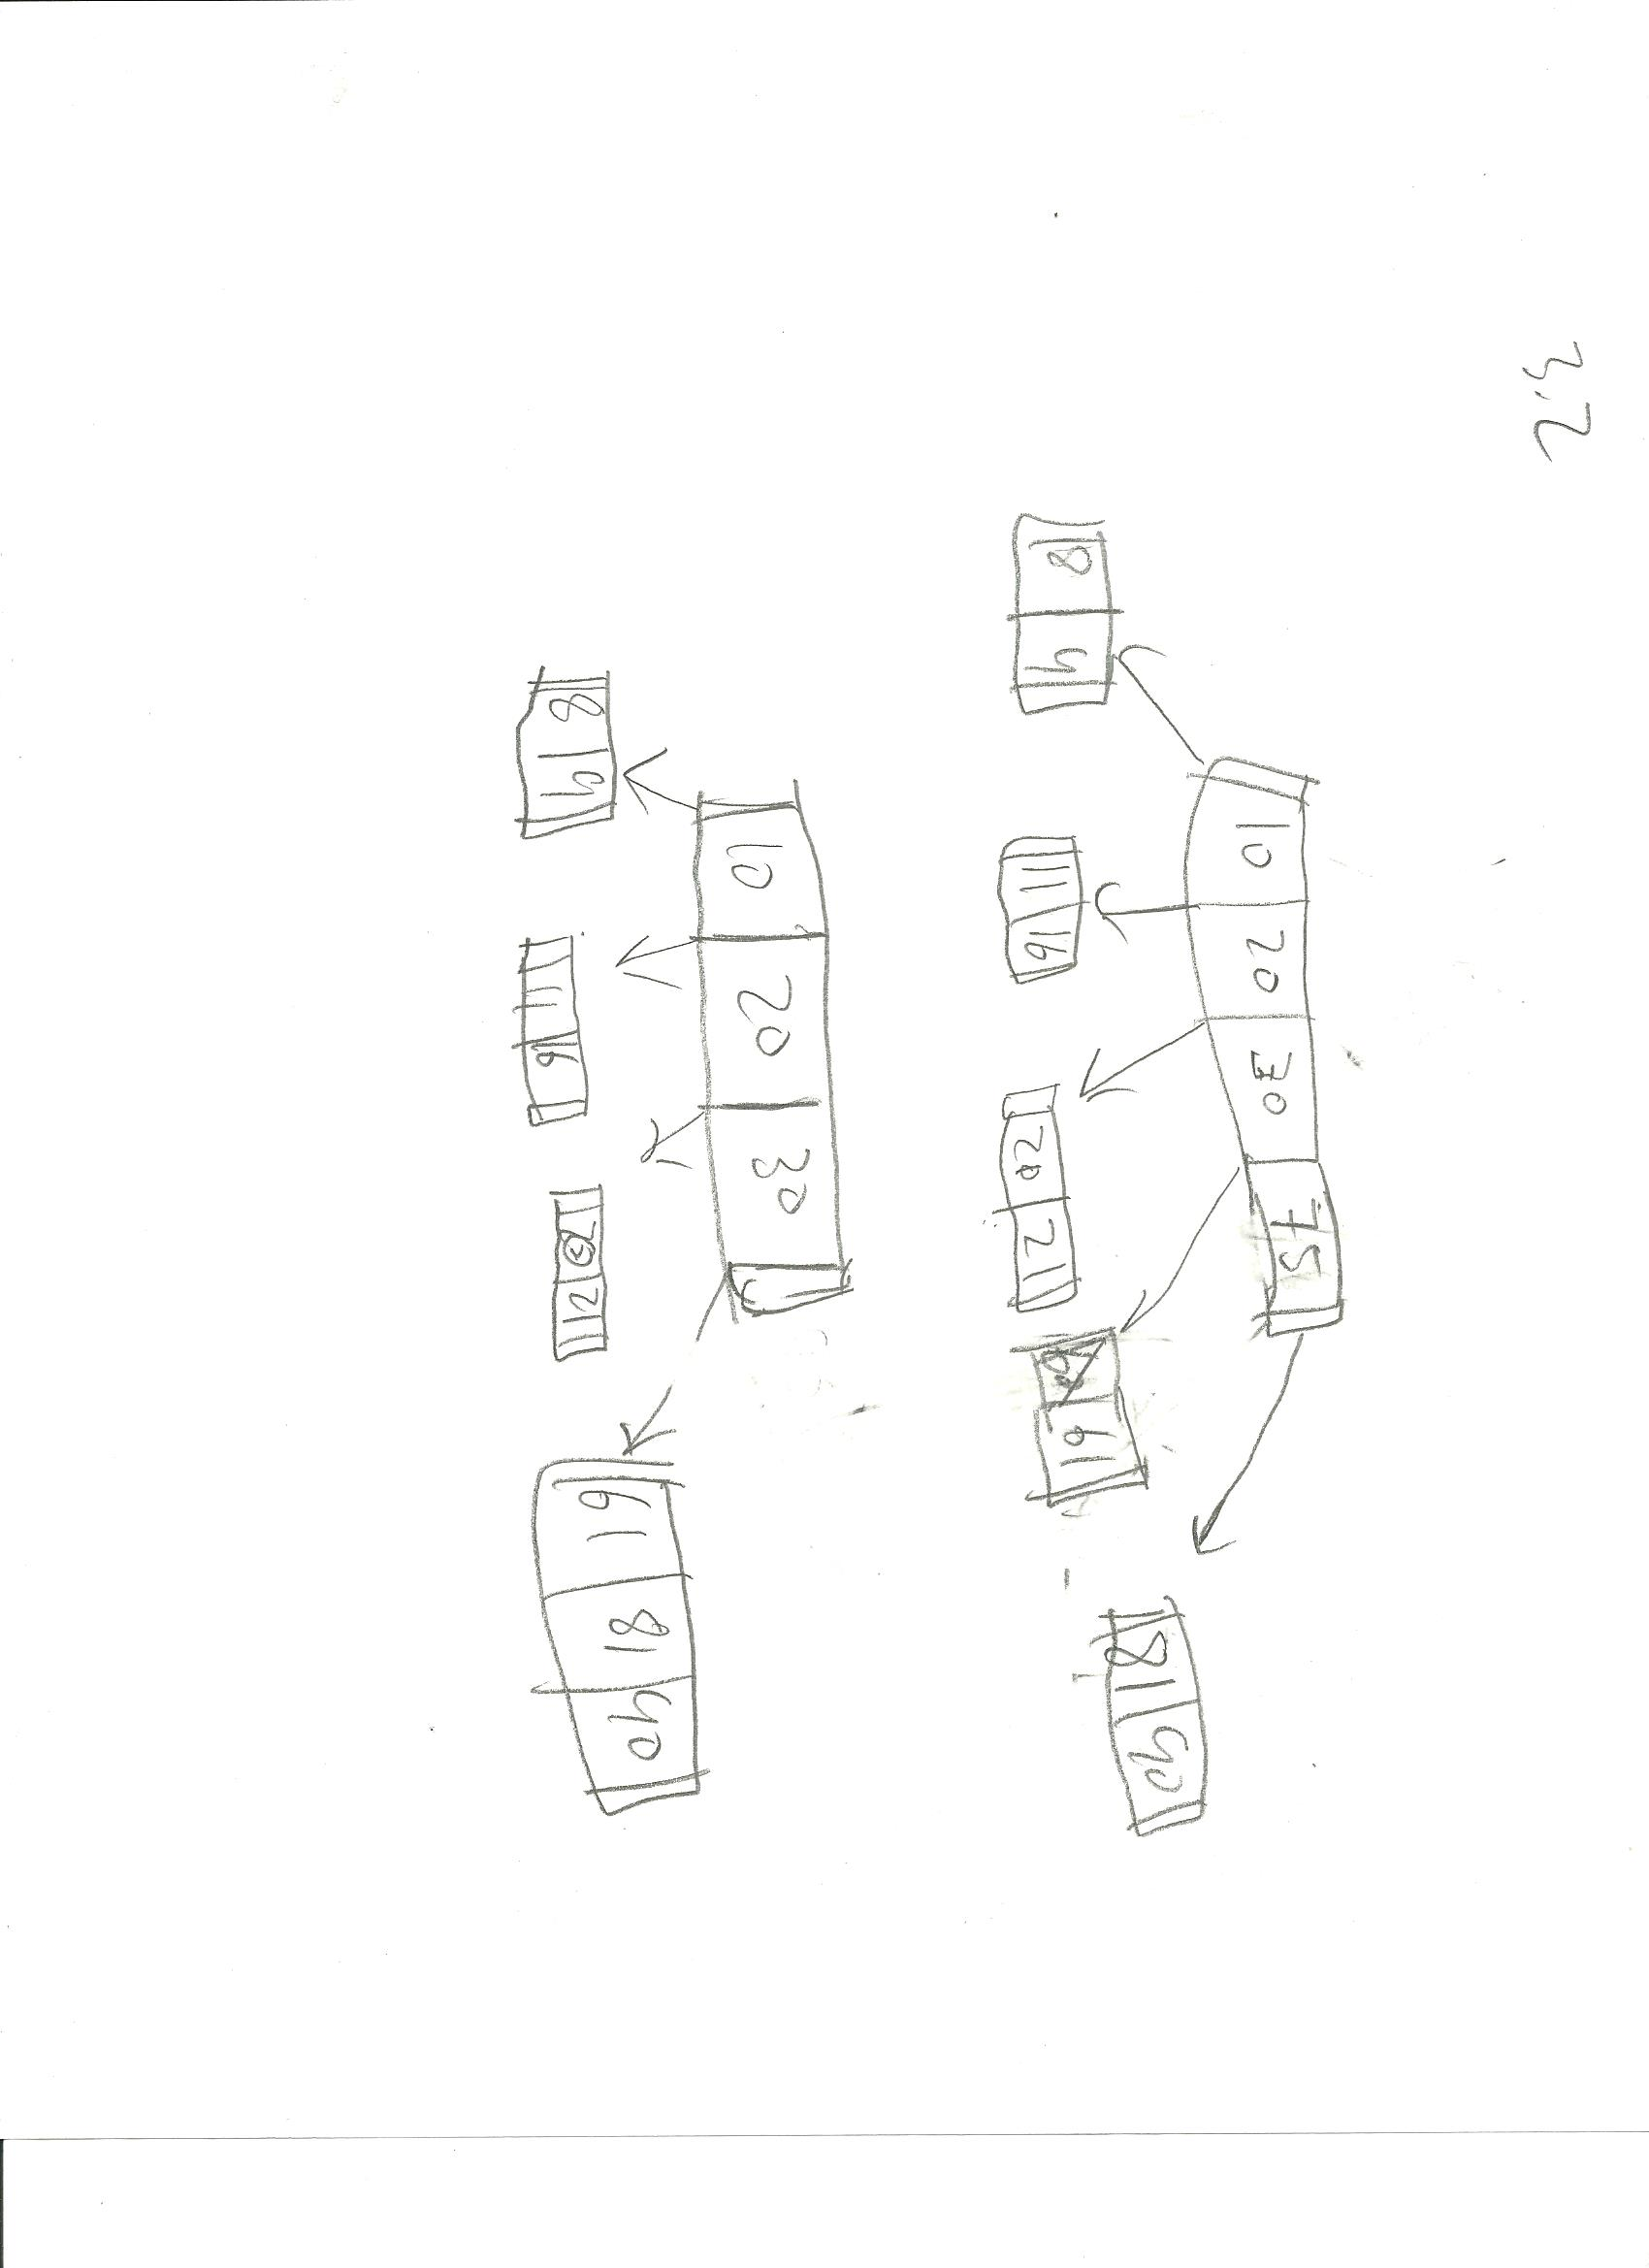
\includegraphics{threePointTwo.jpeg}
	

%	\item A B+ tree in which the deletion of the value 25 causes a merge of two nodes but without altering the height of the tree.
\end{enumerate}


\question{4}{B+ Tree Indexing (1 point)}
Consider the instance of the Students relation shown in Figure~\ref{figure:q4}. 
%Show a B+ tree of degree 2 in each of these cases below. 
\begin{enumerate}
	
	\item To reduce the number of I/O access in index search, each B+ tree node should fit in a block. Let {\it sid} be an integer requiring 16 bits. Let a pointer require 32 bits.
	If the block size is 28 bytes (consisting of 8 bits), what is the maximum degree of the B+ tree index on {\it sid} so each B+ tree node fit in a block?
	
	\paragraph{Solution:} \hfill \break
	Shown below is an equation for the block size given the Key size and the Record pointer size. We will use this to solve this problem.\\
	
\begin{multline}
	k_v = Key Value size \\
	r_p = Record pointer size \\
	b_s = block size \\
	d = degree\\
	2d k_v + (2d + 1) r_p <= b_s 
\end{multline}
	Given this equation and the values given in the question prompt we can say the follow:\\
	
	\begin{multline}
		2d * 16 + (2d + 1) * 32 <= 28 * 8\\
		32d + 32*(2d + 1) <= 224\\
		d + (2d + 1) <= 7\\
		3d <= 6\\
		d <= 6
	\end{multline}
	As shown by the equation above the degree of this tree can be no larger than 2.\\
	

	\item Show a B+ tree index on {\it sid} of degree calculated in part 1 for all records in Figure~\ref{figure:q4}.
	
	solution shown below in figure.\\
	
	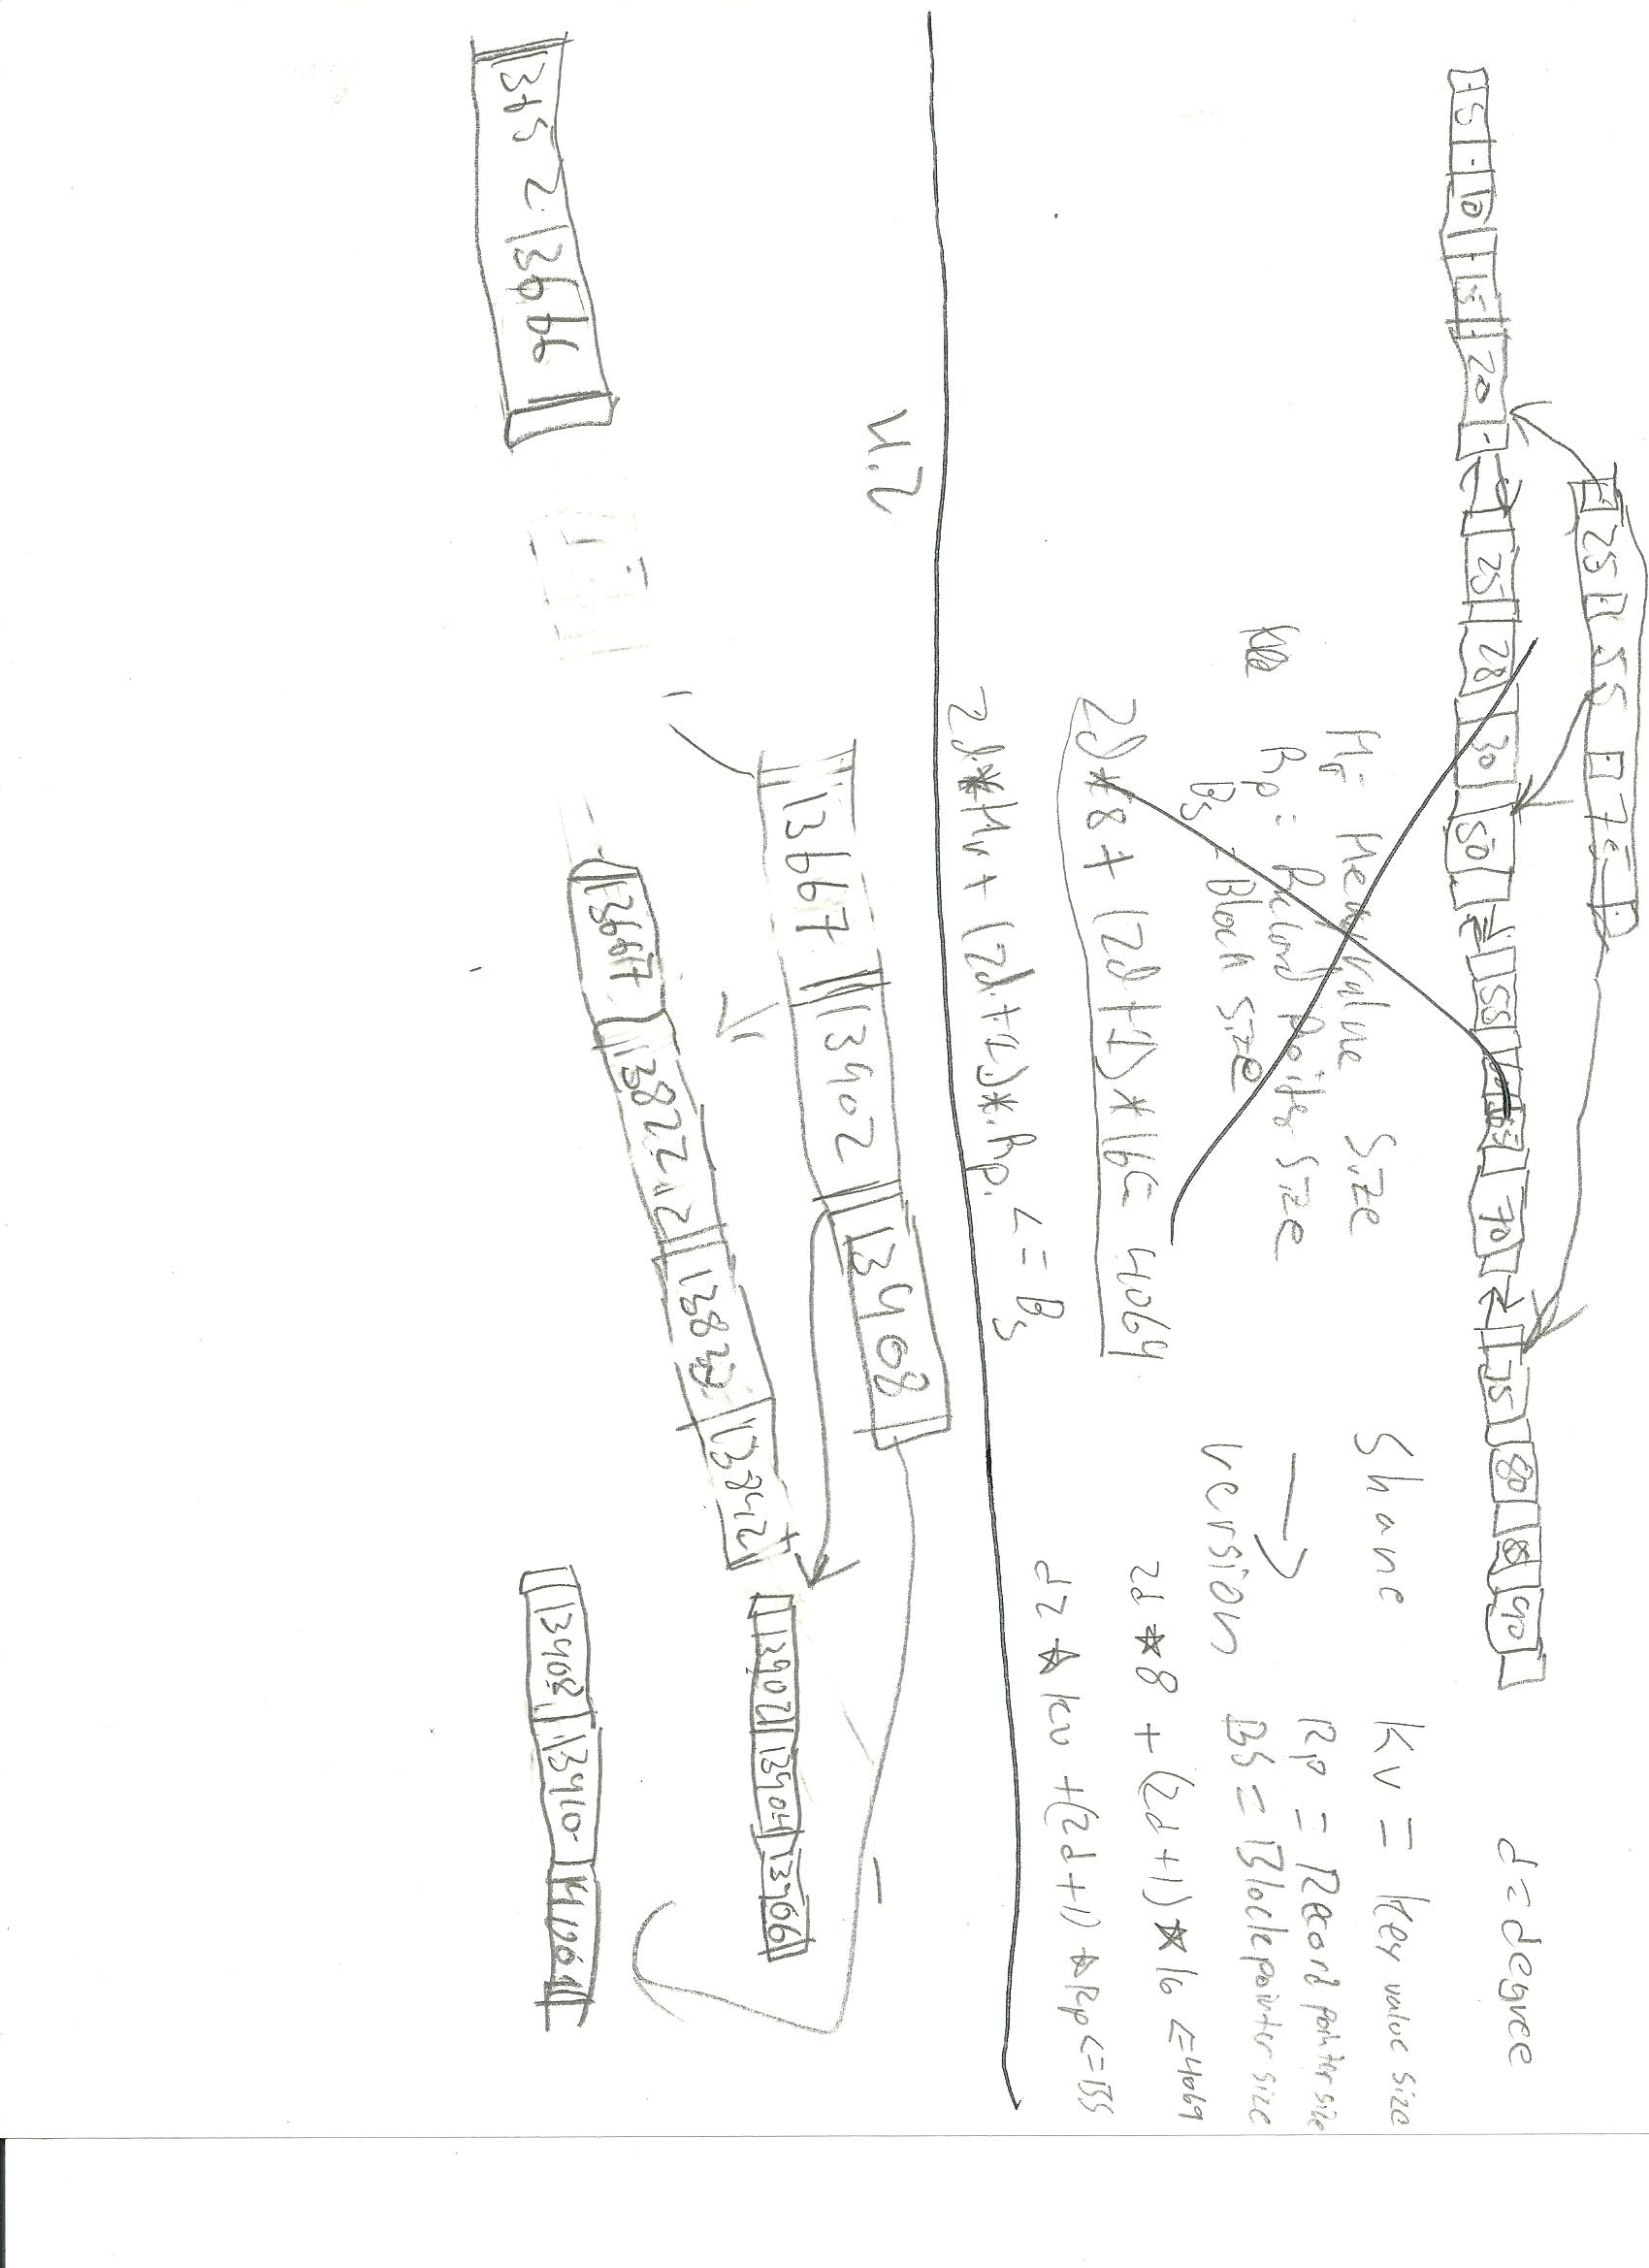
\includegraphics{fourPointTwo.jpeg}


	
	
	
%	\item A dense B+ tree index on {\it gpa} where leaf nodes contain
%	the search key and a pair $\left\langle \mathit{pageid}, \mathit{slot} \right\rangle$ to identify a tuple.
%	For this question, assume that these tuples are stored in a sorted file in the order shown in Figure~\ref{figure:question_3}: The first tuple is in page 1, slot 1; the second tuple is in page 1, slot 2; and so on. Each page can store up to {\bf three} data records. 
%	For example, the first tuple is represented by ``1.8: $\left\langle 1,1 \right\rangle$''.

\end{enumerate}







\end{document}
